\starthis\section[低能散射]{低能散射$^{*}$} \label{sec:08.03} % 
% \makebox[5em][s]{} % 短题目拉间距
% \starthis 章节加星

继续上节的讨论,设散射作用势$V(r)$是短程的,在作用球(半径$a$)以外$V\approx0$.令$E=\frac{\hbar^{2}k^{2}}{2\mu}$,并考虑低能散射,$ka\ll 1$.这时第$l$级分波相移$\delta_{l}$大致与$(ka)^{2l+1}$成比例.[参看\eqref{eq82.26}式和\eqref{eq82.35}式,以及刚球散射.]可以只考虑s波$(l=0)$散射,而略去其他分波$(l\geqslant1)$的贡献.s波径向方程为
\begin{empheq}{equation}\label{eq83.1}
	\frac{d^{2}}{dr^{2}}u_{0}+\bigg[k^{2}-\frac{2\mu}{\hbar^{2}}V(r)\bigg]u_{0}=0
\end{empheq}
取低能极限$E\rightarrow0(k\rightarrow0)$,并研究$r>a$处(作用球外)$u_{0}$的表现形式.这时$V\approx0$,\eqref{eq83.1}式成为
\eqshort
\begin{empheq}{equation}\label{eq83.2}
	\frac{d^{2}}{dr^{2}}u_{0}=0
\end{empheq}
解为
\begin{empheq}{equation}\label{eq83.3}
	u_{0}(r)=c\bigg(1-\frac{r}{a_{0}}\bigg)
\end{empheq}\eqnormal
$c$及$a_{0}$为常数,$a_{0}$称为“散射长度”,其意义稍后再加以说明.

根据\eqref{eq82.11}式,在作用球外应该有渐近形式
\begin{empheq}{align*}
	u_{0}(r) &\approx A_{0}\sin(kr+\delta_{0})	\\
	&=A_{0}\sin\delta_{0}(\cos kr+\cot\delta_{0}\cdot\sin kr)
\end{empheq}
在低能极限下,$k\rightarrow=,\cos kr\rightarrow1,\sin kr\rightarrow kr$,上式成为
\begin{empheq}{equation*}
	u_{0}(r) \approx A_{0}\sin\delta_{0}(1+kr\cot\delta_{0})
\end{empheq}
与\eqref{eq83.3}式比较,可知
\begin{empheq}{equation}\label{eq83.4}
	\boxed{k\cot\delta_{0}=-\frac{1}{a_{0}}\quad(k\rightarrow0)}
\end{empheq}
散射振幅的低能极限为
\begin{empheq}{align}\label{eq83.5}
	f(\theta) &\approx f_{0}=\frac{1}{k}\sin\delta_{0}e^{i\delta_{0}}	\nonumber\\
	&=\frac{1}{k\cot\delta_{0}-ik}=-\frac{a_{0}}{1+ika_{0}}
\end{empheq}
如散射长度$a_{0}$取有限值,则当$k\rightarrow0,k|a_{0}|\ll1$,\eqref{eq83.5}式即
\begin{empheq}{equation}\label{eq83.6}
	f(\theta) \approx-a_{0}\quad (k\rightarrow0)
\end{empheq}
这时\eqref{eq83.4}式给出
\begin{empheq}{equation}\label{eq83.7}
	-ka_{0}=\tan\delta_{0}\approx\sin\delta_{0}\approx\delta_{0}
\end{empheq}
散射截面为
\begin{empheq}{align}\label{eq83.8}
	\sigma(\theta)&=|f(\theta)|^{2}=a_{0}^{2}	\nonumber\\
	\sigma_{\text{总}}&=4\pi a_{0}^{2}
\end{empheq}
这种情况下势场$V(r)$的散射效果相当于半径为$a_{0}$的刚球.注意$\delta_{0}$与$k$成正比,$f(\theta),\sigma(\theta)$均与$k$无关,即与能量$E$无关.

如$a_{0}\rightarrow\pm\infty$,则\eqref{eq83.4}式给出
\begin{empheq}{equation}\label{eq83.9}
	k\cot\delta_{0}=0,\quad \delta_{0}=\frac{\pi}{2},\quad\text{或}\quad -\frac{\pi}{2}
\end{empheq}
而\eqref{eq83.5}式给出
\eqshort
\begin{empheq}{equation}\label{eq83.10}
	f(\theta)=\frac{i}{k}
\end{empheq}\eqnormal
因此
\begin{empheq}{equation}\label{eq83.11}
	\sigma_{\text{总}}=4\pi\sigma(\theta)=\frac{4\pi}{k^{2}}=\frac{2\pi\hbar^{2}}{\mu E}
\end{empheq}
散射截面与$E$成反比.当$E\rightarrow0,\sigma_{\text{总}}\rightarrow\infty$,称为“共振散射”.

\begin{figure}[!h]
	\centering
	\small
	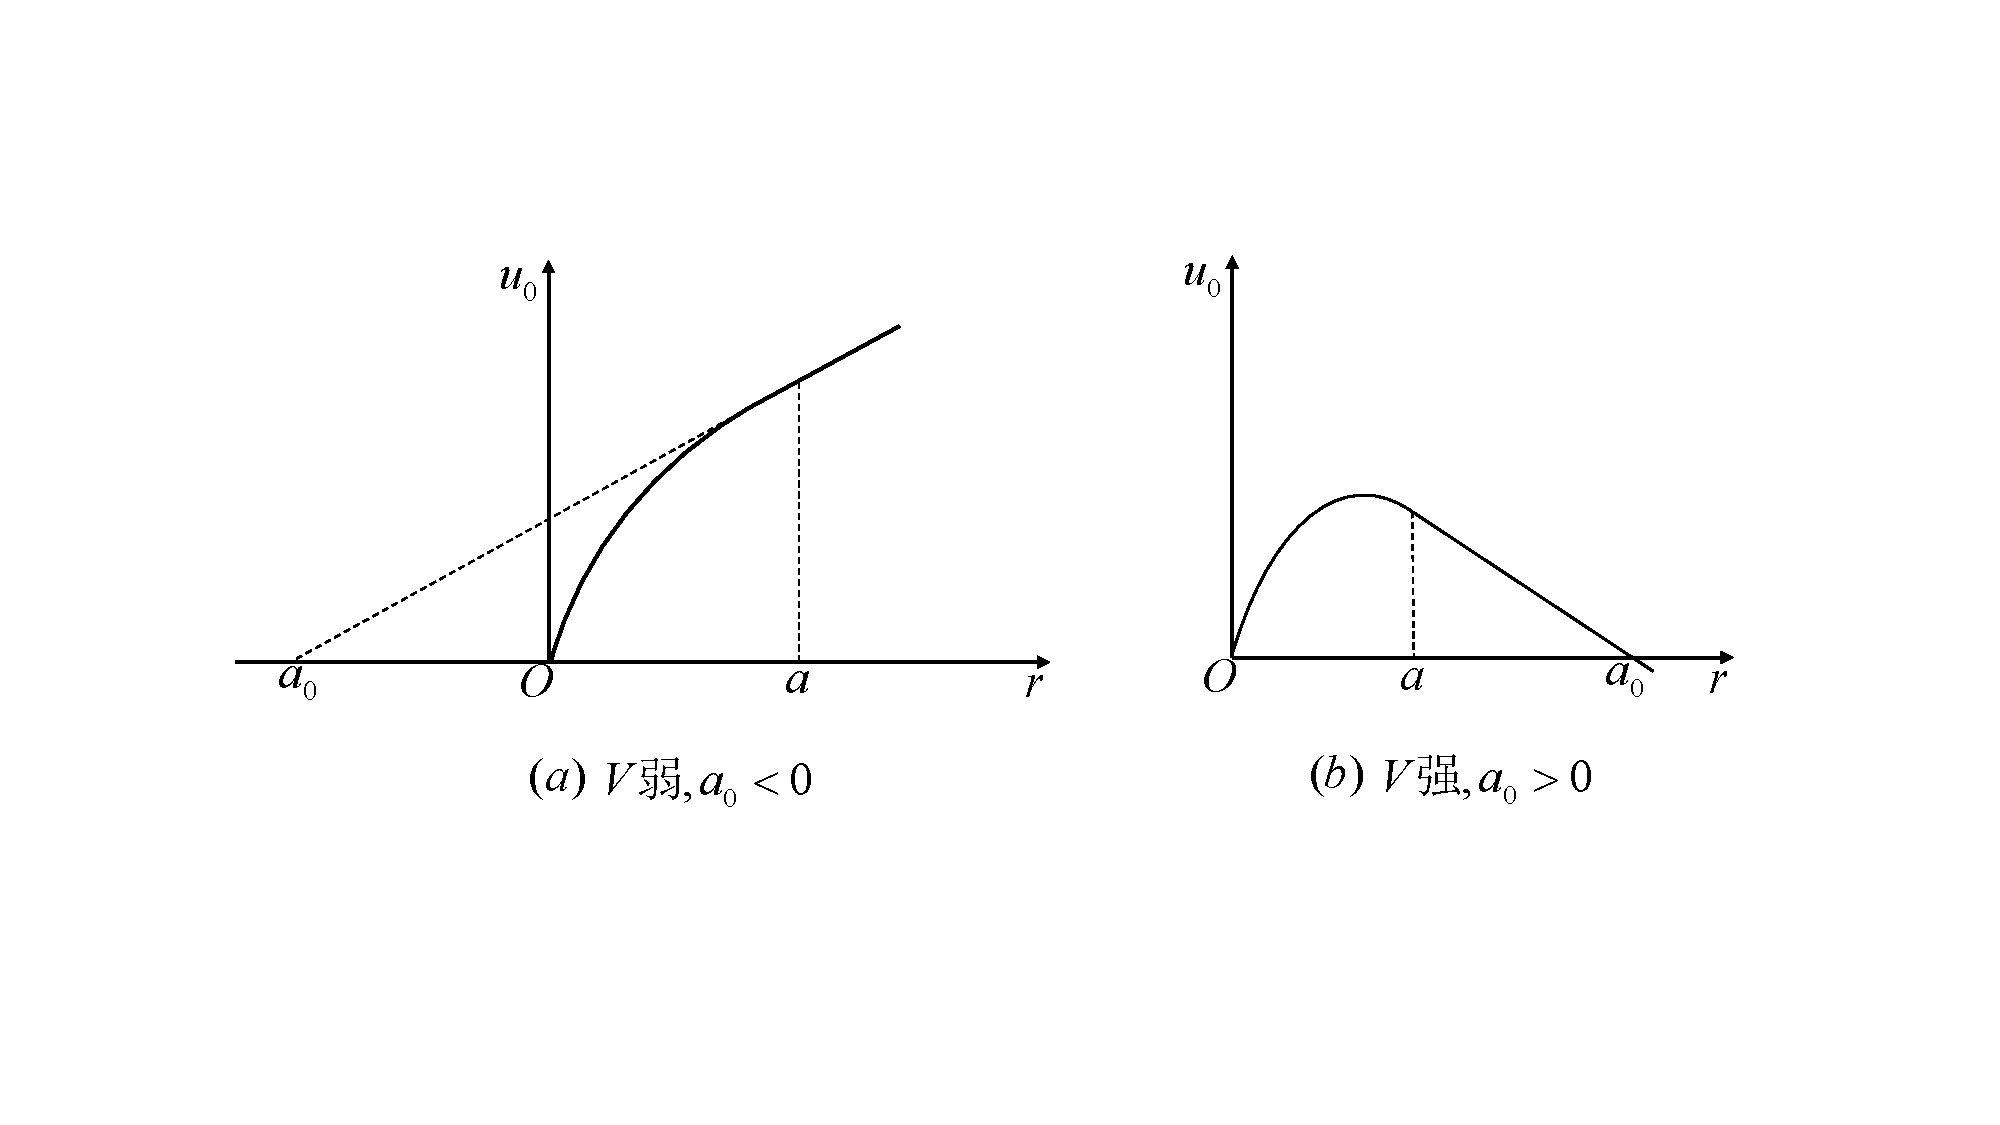
\includegraphics[width=7cm,clip]{QM file/figure/8-4}
	\caption{}\label{fig.8-4}
\end{figure}

下面以势阱$(V<0)$散射为例,说明散射长度的意义.当$E\rightarrow0$,由\eqref{eq83.1}式可知$\frac{u_{0}^{\prime\prime}}{u_{0}}$,$u_{0}$随$r$的变化如图\ref{fig.8-4}所示.如果作用势$V(r)$较弱,以致当$r$达到$a$(作用球半径)时$u_{0}$尚在上升阶段,$u_{0}^{\prime}$为正,则散射长度$a_{0}<0$.这种势阱不能造成束缚态.如果作用势$V(r)$较强,当$r$达到$a$时$u_{0}$已经处于下降阶段,$u_{0}^{\prime}$为负,则散射长度$a_{0}>0$.这种势阱可以造成束缚态能级$(E_{n}<0)$.而$a_{0}=\pm\infty$相当于$r=a$处$u_{0}^{\prime}=0$,这刚好是阱口出现束缚态能级$(E=0_{-})$的条件,这种情况下粒子的入射能量$(E\geqslant0)$接近于阱口附近的束缚态能级,在入射波与阱口束缚态之间容易产生共振跃迁,所以散射截面特别大.
\pskip

\example 讨论球形势阱

\begin{equation}\label{eq83.12}
	V(r)=
	\begin{cases}
		-V_{0},	& r<a	\\
		0,	& r>a
	\end{cases}
\end{equation}
造成的低能$(ka\ll1)$s波$(l=0)$散射.

\solution 令
\begin{empheq}{equation}\label{eq83.13}
	k=\frac{\sqrt{2\mu E}}{\hbar},\quad k_{0}=\frac{\sqrt{2\mu V_{0}}}{\hbar}
\end{empheq}
在阱内$(r<a)$,s波径向方程为
\eqshort
\begin{empheq}{equation}\label{eq83.14}
	u_{0}^{\prime\prime}+(k^{2}+k_{0}^{2})u_{0}=0
\end{empheq}\eqnormal
边界条件为$u_{0}(r=0)=0$.当$E\rightarrow0(k\rightarrow0)$,满足边界条件的解是
\begin{empheq}{equation}\label{eq83.15}
	u_{0}(r)=A\sin k_{0}r\quad (E\rightarrow0,r<a)
\end{empheq}
在阱外$(r>a)$,径向方程为
\eqshort
\begin{empheq}{equation*}
	u_{0}^{\prime\prime}+k^{2}u_{0}=0
\end{empheq}\eqnormal
当$E\rightarrow0$,解为
\begin{empheq}{equation}\label{eq83.16}
	u_{0}(r)=c\bigg(1-\frac{r}{a_{0}}\bigg)\quad (E\rightarrow0,r>a)
\end{empheq}
在$r=a$处,$\frac{u_{0}}{u_{0}^{\prime}}$应该连续,据此求出
\begin{empheq}{align}\label{eq83.17}
	\frac{1}{k}&\tan k_{0}a=a-a_{0}	\nonumber\\
	a_{0}=&-\frac{a(\tan k_{0}a-k_{0}a)}{k_{0}a}
\end{empheq}
$a_{0}$即散射长度.如$a_{0}$有限,由\eqref{eq83.8}式就得到散射截面(与$E$无关).

讨论:(i) 如势阱的性质($V_{0}$及$a$值)刚好使$\tan k_{0}a=k_{0}a$,这时$a_{0}=0$,低能极限下$(E\rightarrow0)\sigma_{\text{总}}\rightarrow0$,势阱是“透明”的.


(ii) 如势阱深而宽,$k_{0}a\gg 1$,同时$\tan k_{0}a$并不太大(非共振散射),这时$a_{0}=a,\sigma_{\text{总}}\approx4\pi a^{2}$,势阱的低能散射效果类似于刚球.


(iii) 如果$k_{0}a=\bigg(n+\frac{1}{2}\bigg)\pi(n=0,1,2,\cdots)$则当$E\rightarrow0$时出现共振散射$(a_{0}=\pm\infty)$.这时阱内区域粒子的德布罗意波长$\lambda_{0}\bigg(\approx\frac{2\pi}{k_{0}}\bigg)$与势阱半径$a$有关系
\eqshort
\begin{empheq}{equation}\label{eq83.18}
	2a=\bigg(n+\frac{1}{2}\bigg)\lambda_{0}
\end{empheq}\eqnormal
这也就是阱口出现束缚能级$(E=0_{-})$的条件.

(iv) 如果势阱浅而窄,$k_{0}a\ll 1$,则可取
\begin{empheq}{equation*}
	\tan k_{0}a\approx k_{0}a+\frac{1}{3}(k_{0}a)^{3}
\end{empheq}
由\eqref{eq83.17}式求得散射长度为
\begin{empheq}{equation}\label{eq83.19}
	a_{0}\approx -\frac{a}{3}(k_{0}a)^{2}=-\frac{2\mu V_{0}a^{3}}{3\hbar^{2}}
\end{empheq}
再由\eqref{eq83.7}式、\eqref{eq83.8}式得出
\begin{empheq}{align}
	\delta_{0}&=-k_{0}a=\bigg(\frac{2\mu V_{0}a^{2}}{3\hbar^{2}}\bigg)ak		\label{eq83.20}\\
	\sigma_{\text{总}}&=4\pi a_{0}^{2}=\frac{16\pi}{9}\bigg(\frac{\mu V_{0}a^{3}}{\hbar^{2}}\bigg)^{2}		\label{eq83.21}
\end{empheq}
如直接利用$\delta_{l}$的近似公式[\eqref{eq82.26}式],也可得到同样的结果.







